 \section{Durchführung}
\label{sec:Durchführung}

\subsection{Aufbau}

In Abbildung \ref{fig:WaermepumpeAufbau} ist die Messapparatur der
Wärmepumpe abgebildet. In beide thermisch isolierte Wasserbehälter werden
jeweils 3 Liter Wasser mit einem Messkolben eingefüllt. Wenn die Behälter an den
Kupferschlangen angebracht
werden, sollte darauf geachtet werden, dass sie gut abgedichtet sind, um den
Wärmeaustausch mit der Umgebung gering zu halten. Die Rührmotoren dienen zur
gleichmäßigen Verteilung der Wärme in den Reservoiren.
Der Kompressor wird durch einen Motor angetrieben, der am Netz angeschlossen
ist. Parallel zu dem Motor ist ein Wattmeter geschaltet, mit welchem die
mechanische Leistung gemessen werden kann. Mit Hilfe einer elektrischen Uhr
wird die Zeit gemessen.

\newpage

\begin{figure}
  \centering
  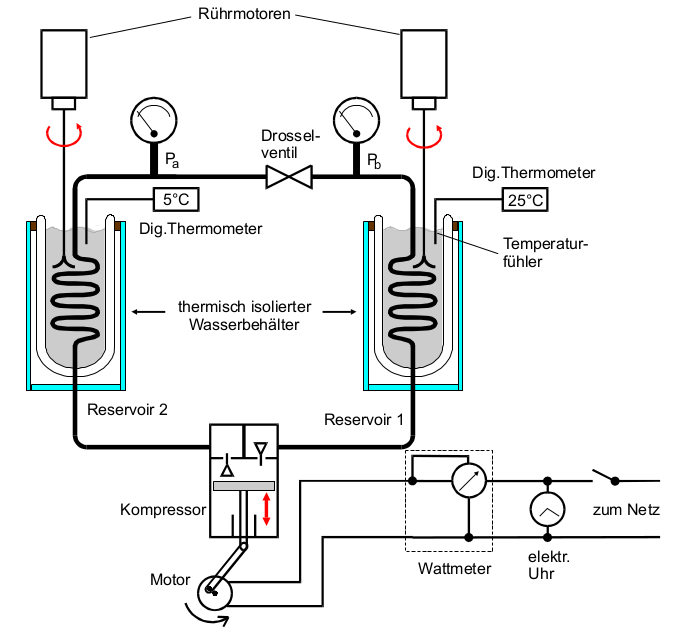
\includegraphics[height=11cm]{WaermepumpeAufbau.png}
  \caption{Messapparatur der Wärmepumpe.\cite{anleitung}}
  \label{fig:WaermepumpeAufbau}
\end{figure}

Folgende Werte sind durch die Apparatur gegeben:
\begin{align}
  & \text{Spezifische Wärmekapazität der Reservoire:} & m_\text{k}c_\text{k} & =\SI{660(10)}
  {\joule\per\kelvin} \\
  & \text{Füllmenge der Reservoire:} & m_1 = m_2 & = \SI{3.000(1)}{\kilo\gram} \\
  & \text{Abweichung der Druckmesswerte:} & \sigma_\text{p} & =\pm \SI{0.2}
  {\bar} \\
  & \text{Abweichung der Temperaturmesswerte:} & \sigma_\text{T} & =\pm
  \SI{0.1}{\kelvin} \\
  & \text{Abweichung der Leistungsmesswerte:} & \sigma_\text{N} & =\pm \SI{5}
  {\watt}
\end{align}

\subsection{Messablauf}

Beim Ablesen der Drücke am Manometer muss der Normaldruck von etwa
\begin{equation}
  p_0 = \SI{1}{\bar}
\end{equation}
beachtet werden. Dieser Druck wird zu jedem Messwert hinzugerechnet.
Die Temperaturen werden von den jeweiligen digitalen Thermometern abgelesen.

\begin{enumerate}

\item Nachdem der Versuch aufgebaut wurde, werden die Rührmotoren eingeschaltet.
Dann werden die Startwerte für $p_\text{a}$, $p_\text{b}$, $T_1$ und $T_2$
aufgenommen.

\item Der Strom wird eingeschaltet, sodass der Motor und die Stoppuhr starten.
In einem Abstand von einer Minute, werden die Messwerte für $p_\text{a}$,
$p_\text{b}$, $T_1$, $T_2$, die Zeit $t$ und die Kompressorleistung $N$ notiert.

\item Die Messung wird bei der Temperatur
\begin{equation}
  T_1 = \SI{50}{\celsius}
\end{equation}
beendet.

\end{enumerate}
